\SetKw{State}{state}
\SetKw{Send}{send}
\SetKw{Wait}{wait}
\SetKw{Call}{call}
\SetKw{Return}{return}

\SetKwComment{Comment}{//}{}

\SetKwProg{Function}{function}{}{end}

\SetKwBlock{parallelblk}{Do In Parallel}{end}
\SetKwBlock{atomicblk}{atomic}{end}

\SetKwFunction{atomicincr}{AtomicIncrement}
\SetKwFunction{atomicdecr}{AtomicDecrement}
\SetKwFunction{clientSubmit}{Client::SubmitOps}
\SetKwFunction{leaderSubmit}{Leader::SubmitOpRecv}
\SetKwFunction{replicaCoord}{Replica::coordRequestRecv}
\SetKwFunction{detectConf}{Leader::DetectConflicts}
\SetKwFunction{detectConfAtLeader}{DetectConflicts}
\SetKwFunction{append}{.append}
\SetKwFunction{pop}{.pop()}

\algnewcommand{\IfThenElse}[3]{% \IfThenElse{<if>}{<then>}{<else>}
  \algorithmicif\ #1\ \algorithmicthen\ #2\ \algorithmicelse\ #3}

\algnewcommand{\IfThen}[2]{% \IfThenElse{<if>}{<then>}{<else>}
  \algorithmicif\ #1\ \algorithmicthen\ #2}

% \section{MDL Protocol}
% \label{sec:design}
% 1. what are the key features it needs to do. which component of the protocol does that.
% 2. include parts in the motivation that describe why you can't simply do "X". and then in design you can refer to motivation...
% 3. map the definition to the instantiation that satisfies this defintion
% 4. top level -- per client, and total order
% We need to guarantee
% (1) in order at each shard per client --> seqnos
% (2) commit order of reqs in a batch across shards --> intershard communication
% (3) consistent interleavings of concurrent batches from separate clients --> reordering
% (4) need correct reordering, so as not to incur other incorrect interleavins --> version number
% (5) need to ensure logs at multiple shards aren't attempting to reissue, and end up in another state with incorrect interleavings --> Use PID

\mdl is an extension of \sdl that allows per-client concurrency. To get the most performance from \md, ideally we want to issue all available outstanding requests from each client in parallel to each shard. To ensure safety, we have to guarantee (1) issue-order for each individual client, and we have to guarantee (2) a total order across all clients that respects each client's issue-order.

\begin{figure}[!htb]
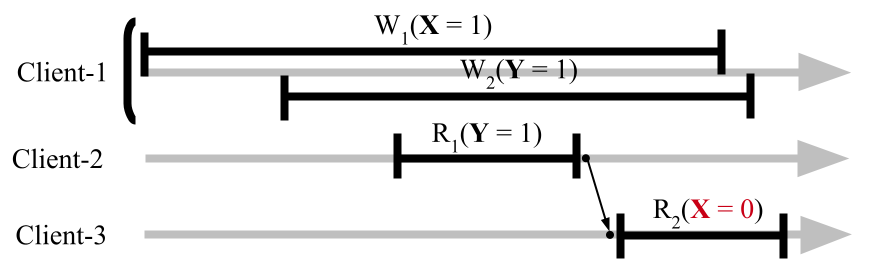
\includegraphics[scale=.45]{invocation_ordering_across_shards.png}
\caption{To provide invocation orderacross shards, an \md protocol requires some intershard coordination. Otherwise, concurrent requests can execute out of order at different shards. In this example execution, Client-1 submits $W_1$ and $W_2$ to shards \textbf{X} and \textbf{Y}, respectively. If a separate Client-2 exposes the completion of $W_2$, all other clients must see the completion of $W_1$. But without intershard coordination, it is possible Client-3 sees an incorrect value for $R_2$.}
\label{fig:invOrdAcrossShards}
\end{figure}

\begin{figure}[!htb]
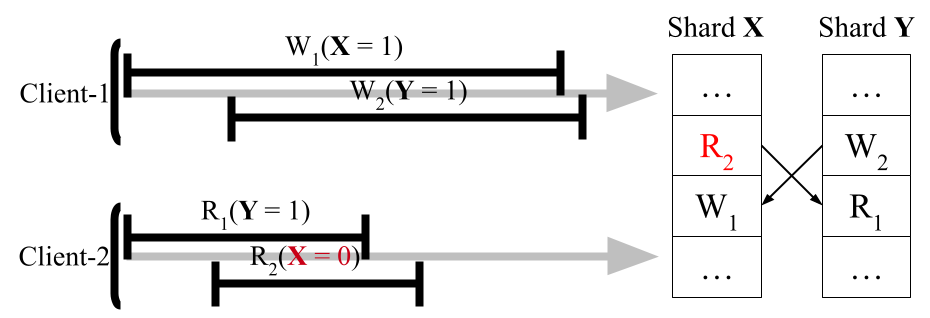
\includegraphics[scale=.45]{somet.png}
\caption{Example execution where two concurrent clients each submit 2 concurrent requests. Assume keys \textbf{X} and \textbf{Y} are at different shards. It is possible that $R_2$ arrives before $W_1$ at shard \textbf{X}, and $W_2$ arrives before $R_1$ at shard \textbf{Y}. Since clients expect their concurrent requests to take affect in invocation order, if $R_1$ returns 1, then $W_1$ must have taken affect before $R_1$, so $R_2$ should necessarily return a value of 1.}
\label{fig:concurrentbatches}
\end{figure}

\subsection{Issue Order Per Clients}
We use per-client sequence numbers to guarantee invocation order for each client at each individual shard. The sequence numbers must be be numbered individually with respect to each shard, for example, a client issuing requests to two different shards for the first time will submit two requests both with sequence number 0. If a shard leader receives a request from a client with a different sequence number than it is expecting for them, it buffers the out of order request until requests with the expected sequence numbers arrive and are committed in order.

As shown in figure \ref{fig:invOrdAcrossShards}, using sequence numbers provides invocation at each shard, but it is not enough to provide invocation order across shards. \sdl does not require inter-shard coordination, since concurrent requests to separate shards can only come from independent clients and require no inter-client ordering. For \mdl however, it is possible that concurrent requests get committed at different shards in an order inconsistent with invocation order if the client issues everything in parallel. Inter-shard coordination between shards is thus necessary for \md. Moreover, this shows intuitively why \mdl, unlike \sdl, is not composable (or local).

One potential approach to guarantee issue-order across shards would be for the leader at each shard to block on committing a request until it receives coordination messages that indicate any concurrent requests invoked earlier at other shards by the same client have been committed first. This general inter-shard coordination handles the case demonstrated in figure \ref{fig:invOrdAcrossShards} and more generally gives us requirement (1). Unfortunately, this is not enough to also provide requirement (2), as we will discuss in the next section.

\subsection{Total Order}
To ensure a total order of requests across all clients that respects each client's invocation order, \mdl must guarantee consistent interleavings of concurrent batches from separate clients. Figure \ref{fig:concurrentbatches} shows how concurrent clients can submit 2 concurrent requests across different shards and end in a state that does not respect \mdl. Unlike figure \ref{fig:invOrdAcrossShards}, figure \ref{fig:concurrentbatches} shows that ensuring each individual client's concurrent requests are committed in invocation order across shards is not strong enough to provide \mdl, there must be a consistent ordering across clients as well.

We denote the final state depicted in \ref{fig:concurrentbatches} as a conflict state. A conflict may occur in an execution when (1) there are at least two concurrent clients each submitting concurrent requests, (2) there are at least 2 shards involved, (3) globally, at least two operations in flight are writes to at least 2 different shards (4) $|(\bigcup\limits_{w \in \mathcal{W}}k_w) \bigcap (\bigcup\limits_{op \in \mathcal{B}}k_{op})| > 1$, and (5) a global key order is not respected by clients issuing concurrent requests. 

Intuitively, a conflict occurs when there is a dependency cycle across entries from different clients in the logs of at least more than 1 shard. The dependencies derive from two sources. The first is the invocation order that each client expects, since each request issued depends on previously issued requests taking effect before it does, and the log order that each shard assigns based on when requests arrive and get replicated. 

% (4) you'll never get a conflict if all shards have reads and only one shard has some ordering of writes
Discussion on interleavings and how there are many more that are correct over how many are incorrect --> inspires optimistic protocol. Conflicts should be rare, especially given a large keyspace and multiple shards. This motivates an optimistic approach where we do not enforce a single correct ordering.

\subsubsection{Conflict Detection}
\subsubsection{Log Reordering}

(2) need correct reordering, so as not to incur other incorrect interleavings; (3) need to ensure logs at multiple shards aren't attempting to reissue, and end up in another state with incorrect interleavings.

Discussion on assigning version number -- optimization is to treat reads as not changing version number, but if not op agnostic you don't have to do this, but there will be false positives (think it's inconsistent and reorder to get correct state, but initial state didn't appear to clients as incorrect).


\begin{enumerate}
    \item client sends request[(Op,Key,Value), PID, seqno, batchdependencies] to shard leader responsible for that key
    \item if this is not the next expected sequence number from this pid, buffer the request in memory
    \item shard leader creates entry for request: [(Op,K,V), PID, seqno, batchDeps, initialLD=propagatedBD, newLD=nil]
    \item propagatedBD := append(propagatedBD, batchDeps)
    \item sends Accept to all replicas
    \item sends Intershard to all shard leaders, for each batch dependency
    \item check to see if there are any outstanding buffered entries, if so repeat steps 3-6 for each of these
    \item Once we've received a quorum of Accept replies and ALL of our Intershard replies, detect conflicts
    \item if no conflicts detected, commit entry and respond to client
    \item else reorder the entry after the conflict with the highest index, make sure to push all the entries between you and the index you're moving to that come from the same PID and operate on the same key
    \item sends Reorder to all replicas
    \item once we've received a quorum of Reorder replies, commit entry and respond to client
    \item once an entry gets committed, remove its batchdependencies from propagatedBD
\end{enumerate}


%%%%%%%%%%%%%%%%%%%%%%%%%%%%%%%%%
%%%%%%%%% Client %%%%%%%%%%%%%%%%
%%%%%%%%%%%%%%%%%%%%%%%%%%%%%%%%%
\begin{algorithm}
    \State $PID \gets$ unique client ID\\
    \State $\mathcal{L} \gets \{...\}$ \algorithmiccomment{Shard Leaders}\\
    \State $s \gets \{0,...,0\}$ \algorithmiccomment{Sequence No Per Shard}\\
    \Function{\clientSubmit{Ops, Ks, Vs}}{
        $batchDeps \gets nil$\\
        \For{$K \in Ks$}{   
            $Req \gets (Ops_K, K, V_K, PID, s_{L_K}, batchDeps)$\\
            \Send $SubmitOp(Req)$ to $L_K \in \mathcal{L}$\\
            $batchDeps\append{Req}$\\
            $s_{L_K} \gets s_{L_K}+1$\\
        }
        
        \Wait receive $SubmitOpReply(V)$ from $L_K \in \mathcal{L}$ for all $K \in Ks$\\
        }
    \caption{MD-Lin Client}
\end{algorithm}
%%%%%%%%%%%%%%%%%%%%%%%%%%%%%%%%%
%%%%% Shard Leader %%%%%%%%%%%%%%
%%%%%%%%%%%%%%%%%%%%%%%%%%%%%%%%%
\begin{algorithm}
    \State $pd \gets nil$ \algorithmiccomment{Propagated dependencies}\\
    \State $log \gets nil$ \algorithmiccomment{Request log}\\
    \State $version \gets \{0,...,0\}$ \algorithmiccomment{Per Key}\\
    \State $expectedSeqno \gets \{0,...,0\}$ \algorithmiccomment{Per PID}\\
    \State $buff \gets \{nil,...,nil\}$ \algorithmiccomment{Per PID}\\
    \Function{\leaderSubmit{Op, K, V, P, s, bd}}{
    \eIf{$s \neq expectedSeqno_{PID}$}
    {
    $buff_{PID}(\{Op, K, V, P, s, bd\})$
    }
    {
    \Repeat{$\{Op, K, V, P, s, bd\} = buff_{PID}\pop \neq nil$}
    {
        $ld \gets pd$ \algorithmiccomment{log dependencies}\\
        $pd\append{bd}$\\
        $version \gets version_K$\\
        \IfThen {$Op = \text{WRITE}$}
        {$version_K \gets version_K+1$}\\
        $entry \gets \{Op, K, V, P, s, version, bd, ld\}$\\
        $log\append(entry)$\\
        \Send $AppendEntries(entry)$ to all $r \in \mathcal{R}$\\
        \Send $GetLogDeps$ to $L_k \in \mathcal{L}$ for all $k \in bd$\\
        \Wait receive $AppendEntriesSuccess$ from all $r \in Q \in \mathcal{R}$\\
        \Wait receive $GetLogDepsReply(D_k)$ from all $L_k \in \mathcal{L}$\\ 
        $deps \gets \bigcup_{k \in bd}D_k$\\
        \Call \detectConfAtLeader{entry, deps}\\
        \Send $CommitEntry$ to all $r \in \matchal{R}$\\
        $V \gets execute(entry)$\\
        \Send $SubmitOpReply(V)$ to $client_{PID}$\\
    }
    }
    }
    \Function{\detectConf{me, deps}}{
        $newIndex \gets nil$\\
        \For{$d \in deps$}{   
            \If{$d.k == me.k 
            \\& \land d.version \ge me.version
            \\& \land d.PID > me.PID 
            \\& \land d.index > me.index
            \\& \land d.index > newIndex$}
            {
                $newIndex \gets d.index$
            }
        }
        \IfThen{$newIndex == nil$}{\Return}\\
        \Send $reorderInLog(me, newIndex+1)$ to all $r \in \mathcal{R}$\\
        \Wait receive $reorderInLogSuccess$ from all $r \in Q \in \mathcal{R}$\\
    }
    \caption{MD-Lin Shard Leader}
\end{algorithm}

\subsection{Correctness}

\subsubsection{Leader Failure}